%%%%%%%%%%%%
%
% $Autor: Wings $
% $Datum: 2019-03-05 08:03:15Z $
% $Pfad: Functions.tex $
% $Version: 4250 $
% !TeX spellcheck = en_GB/de_DE
% !TeX encoding = utf8
% !TeX root = manual 
% !TeX TXS-program:bibliography = txs:///biber
%
%%%%%%%%%%%%

\chapter{Funktionen}
\label{sec:Funktionen}
In diesem Kapitel werden die Grundfunktionen des Tischförderbands und deren Konfiguration erläutert.
Weiterhin werden noch erweiterte Funktionen des Systems und ihre Verwendung dargestellt.

\section{Grundfunktionen}

\begin{itemize}
	\item \textbf{Ein- und Ausschalten} \\
	Das \textbf{Tischförderband} ist stehts über den \textbf{Hauptschalter} ein- und auszuschalten. Ziehen Sie niemals das \textbf{Netzteil} im laufenden Betrieb aus der Steckdose oder die \textbf{DC-Buchse} aus dem \textbf{Bedienelement}.
	Im Notfall ist der \textbf{Hauptschalter} als Not-Aus zu verwenden.\\
	\\
	Hinweise zur Inbetriebnahme nach Einschalten des \textbf{Hauptschalters} finden Sie im Abschnitt \ref{sec:Inbetriebnahme}  \textbf{Inbetriebnahme}.
	
	\item \textbf{Anzeige} \\
	Auf der integrierten \textbf{Anzeige} werden dem Benutzer wichtige Meldungen und Betriebsinformationen angezeigt. 
	Bei jedem Einschaltvorgang zeigt die \textbf{Anzeige} kurz den Startbildschirm mit der \textbf{Firmware-Version} und wechselt nach der \textbf{Freigabe der Lichtschranken} in das Hauptmenü (siehe Kapitel \ref{sec:Inbetriebnahme}). 
	
	\textbf{Elemente im Hauptmenü:}
	\begin{enumerate}
		\item Modus
		\item Status der Lichtschranken
		\item Bandgeschwindigkeit
		\item Systemmeldungen / Fehlercodes
		
	\end{enumerate}
	
	%Hier Bild von Anzeige
	\begin{center}
		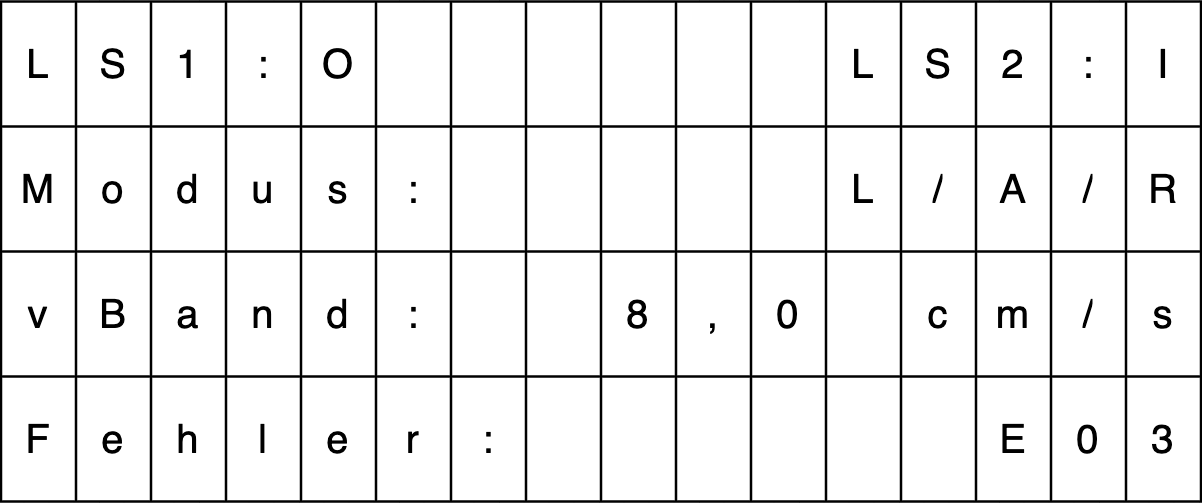
\includegraphics[width=10cm]{NewFiles/Images/Bild_Platzhalter_Anzeige}
	\end{center}
	
	Wird der \textbf{Modus} gewechselt, so wird auf der \textbf{Anzeige} der gewählte Modus für einige Sekunden eingeblendet.
	Anschließend wechselt die \textbf{Anzeige} wieder in das Hauptmenü.
	%{wichtig im Programm ergänzen}
	  
	\item \textbf{Modus / Förderrichtung wählen} \\  
		\begin{itemize}
		\item \textbf{Linkslauf:}
		In diesem Modus erkennt das System, ob in Lichtschranke 2 eine Transportbox abgelegt wurde und transportiert diese zur linken Seite des Tischförderbands bis sie das Transportband verlässt.
			
		Dieser Modus kann zum automatischen Weitertransport einer Transportbox in einen Behälter oder auf ein zweites Tischförderband verwendet werden. Wenn kein weiteres Transportband oder ein Behälter am Ende des Transportbands steht sollte im Abwurfbereich eine weiche Unterlage platziert werden, um die Transportbox nicht zu beschädigen. 
		
		\textbf{Bewegungsablauf:}
		Stellen Sie zunächst den Modusschalter auf \fbox{L}.
		
		
		
		
		
		Wird die Lichtschranke durch ein Objekt unterbrochen, fährt das Transportband mit der voreingestellten Bandgeschwindigkeit an. Das Transportband bewegt sich so lange bis die zweite Lichtschranke unterbochen wird und kommt zum stehen, sobald diese wieder freigegeben wird und das Objekt das Transportband verlassen hat.\\
			
		\item \textbf{Rechtslauf:}
		Im Modus Rechtslauf verhält sich das Tischförderband umgekehrt zum Modus Linkslauf. Die grundlegenden Funktionen und Bewegungsabläufe sind jedoch identisch.
		
		
		
		
		
		\item \textbf{Automatiklauf:}
		In diesem Modus erkennt das System, ob an einem Ende des Transportbandes ein Objekt abgelegt wurde und transportiert dieses bis zum anderen Ende des Transportbandes und verweilt dort.
			
		Dieser Modus kann zum automatischen Weitertransport von Objekten in zwei Richtungen verwendet werden. Eine einfache Sortierstraße ist ebenfalls realisierbar.
			

		
		Wird die erste Lichtschranke durch ein Objekt unterbrochen, fährt das Transportband mit der voreingestellten Bandgeschwindigkeit an. Das Transportband bewegt sich so lange bis die zweite Lichtschranke unterbochen wird und kommt zum stehen.\\
		
		Das System setzt sich nach einer bestimmten Ruhezeit automatisch zurück. Nach ablauf dieser Ruhezeit kann erneut ein Objekt zwischen eine der Beiden Lichtschranken gelegt werden.\\
		
		Das Transportband versucht die Bandgeschwindigkeit unabhängig von der Belastung beizubehalten.\\
		
		Sollte das Objekt die zweite Lichtschranke innerhalb eines festgesetzten Zeitraumes von maximal 30 Sekunden nicht erreichen, hält das Transportband selbstständig an. Auf der Anzeige erscheint der Fehlercode \fbox{XXX}.
		\end{itemize}
	
	
	
	
	
	
	\item \textbf{Bandgeschwindigkeit einstellen} \\  
	Mithilfe des \textbf{Drehreglers} kann die gewünschte \textbf{Bandgeschwindigkeit} eingestellt werden.
	Im Hauptmenü wird auf der \textbf{Anzeige} die eingestellte \textbf{Bandgeschwindigkeit} \fbox{vBand} angezeigt.
	Die Bandgeschwindigeit kann jederzeit geändert werden und beschreibt die maximale Geschwindigkeit, die das Transportband im Betrieb erreichen kann.
	Einstellbare \textbf{Bandgeschwindigkeiten} finden Sie im Kapitel \ref{sec:Spezifikationen} \textbf{Spezifikationen}.

	\item \textbf{Moduswechsel}\\
	Um den Modus zu wechseln, stellen Sie  den Modusschalter auf eine der drei Positionen \fbox{L}, \fbox{A} oder \fbox{R}.
	Nun wird die jeweils andere Lichtschranke zum aktivieren der Bewegung verwendet.
	Sollte das Transportband bei Änderung des Modus in Betrieb sein, so bremst es langsam bis zum Stillstand ab.
	Die Anzeige bittet Sie nun eventuell noch auf dem Transportband liegende Transportboxen zu entfernen. Wenn das Transportband frei ist können Sie diese Meldung mit dem Quittiertaster bestätigen. 
	Abhängig vom gewählten Modus, kann erneut eine Transportbox in eine der Lichtschranken gestellt werden. Der Betrieb des Tischförderbands wird mit dem gewählten Modus fortgesetzt.
	
\end{itemize}

\section{Erweiterte Funktionen}

\begin{itemize}
	
	\item \textbf{Betrieb mit programmiertem Bewegungsablauf} \\ 
	Sollte für eine Anwendung ein gesonderter Bewegungsablauf gewünscht sein, so kann dieser über die Programmierung des verbauten Microcontrollers angepasst werden. 
	Weitere Informationen dazu finden Sie in der Dokumentation.
	
\end{itemize}

\section{Reset}
Wird der Reset-Taster für mehr als 5 Sekunden betätigt, so wird das Transportband umgehend zum Stehen gebracht. Die Steuerung des Systems wird neu gestartet und kehrt zurück in das Startmenü.\\
Um das Tischförderband wieder in Betrieb zu nehmen, konfigurieren Sie das System erneut wie im Abschnitt \ref{sec:Inbetriebnahme} Inbetriebnahme.